
\ifx\isEmbedded\undefined
\pdfobjcompresslevel 0
\documentclass[a4paper, 12pt]{report}


%
%%\usepackage{comment} % Permet de compiler sans les figures et sans les tables
%%\excludecomment{figure}
%%\let\endfigure\relax
%%\excludecomment{table}
%%\let\endtable\relax

%\usepackage{refcheck} %permet de voir les refs du bib non cit�es

\setlength{\parindent}{0pt} %get rid of indentation in the article
\usepackage{etoolbox} % prevent a Patching '\begin' failed! see https://tex.stackexchange.com/questions/128938/package-etoolbox-warning-patching-begin-failed
%\usepackage{natbib} % pour bibtex \citep (parenthetical) et \citet (textual) (sinon seul \cite marche) a loader avant babel
\usepackage[semicolon,round,sort&compress,sectionbib]{natbib}  %
\usepackage{chapterbib}      
\usepackage[english, french]{babel} %Fran�ais à loader avant caption
\usepackage[T1]{fontenc}

  \usepackage{adjustbox}
\usepackage[affil-it]{authblk} %for affiliation
\usepackage{afterpage} % To include blanck page with command \afterpage{\blankpage}
\usepackage{appendix}

\usepackage{array} %pour les tableaux
\usepackage{amsmath, amssymb} %american mathematical society math style and symbols (amssymb)
\usepackage{amsthm}
\usepackage{blindtext}
\usepackage{booktabs}
\usepackage{breqn} % allow to use dmath environment (automatic break for equations, etc) 
\usepackage{caption} % Needed to jump line in figures titles (caption).
%\usepackage{commath} sais pas pourquoi �a marche pas si je charge �a plante !

\usepackage{dirtytalk} % quote stuff with \say{the text to quote}
\usepackage{empheq} %
\usepackage[official]{eurosym}  %type \euro{} to print a euro
\usepackage{float} % for firgure placement with H option
\usepackage{fancybox}

  \usepackage[top=2cm, bottom=2cm, left=2.5cm, right=2.5cm]{geometry}
  \usepackage[top=2cm, bottom=2cm, left=2.5cm, right=2.5cm]{geometry}
\usepackage{graphicx} %pour ins�rer des images.
 \usepackage[hyperindex=true,
 		     colorlinks=true, 
		     urlcolor=blue,
		     citecolor    = blue, %Couleur des citations (biblio)
    		     linkcolor    = blue, %Couleur des équations. Apparemment, cela sert aussi pour théoreme, Lemme...
 					 ]{hyperref} %permet de mettre des hyper liens (le package url le fait tout seul ? la base)

\usepackage{import}					 



\usepackage{pdflscape}
\usepackage{pdfpages} %allow to select which pdf pages to compile \includepdf[pages={12-15,23,45-49}]{main.pdf} 
\usepackage{spverbatim}
\usepackage{lmodern}%change un peu les lettres pour un truc plus cool, marche peut �tre un peu mieux avec les accents v�rifier � l'occaz
\usepackage{mathrsfs} % allows $\mathscr{ABC}$ to work
\usepackage{setspace} % permet de d�terminer une largeur d'interligne
\usepackage{tikz} % draw graphs
\usetikzlibrary{trees,shapes,snakes}
  \usepackage{subcaption} % to use with subfigures
\usepackage{skull}
\usepackage{url}
\usepackage{verbatim} %Pour ins�rer du code informatique

\usepackage{fancyvrb}
\usepackage{fvextra}

\usepackage{array} %one of the two needed to use thead to break line in tabular
\usepackage{makecell} %one of the two needed to use thead to break line in tabular

\DeclareUnicodeCharacter{20AC}{\euro{}}
\DeclareUnicodeCharacter{2212}{-}
\DeclareUnicodeCharacter{300}{`}
\DeclareUnicodeCharacter{301}{'}

  \newcommand{\hdrule}{\midrule[\heavyrulewidth]}

\newsavebox{\mybox}

\newcommand{\raisedshadowbox}[1]{%
\sbox\mybox{\shadowbox{#1}}%
\raisebox{-0.5\ht\mybox-0.5\shadowsize+0.6ex}{\usebox\mybox}%
}
%%%%%
\providecommand{\tightlist}{%
  \setlength{\itemsep}{0pt}\setlength{\parskip}{0pt}}


\bibliographystyle{chicagoa}


%%%%%%%%%%%%%%%%
%%%Fin biblio %%%%%%%%



%%%%Elispse in tables%%%%%%
\usepackage{tikz}
\usetikzlibrary{fit,shapes.misc}
\newcommand\marktopleft[1]{%
    \tikz[overlay,remember picture] 
        \node (marker-#1-a) at (0,-1ex) {};%
}
\newcommand\markElipseBottomright[1]{%
    \tikz[overlay,remember picture] 
        \node (marker-#1-b) at (0.2,0.3) {};%
    \tikz[overlay,remember picture,thick,dashed,inner sep=3pt]
        \node[draw, ellipse,fit=(marker-#1-a.center) (marker-#1-b.center)] {};%
}
%%%%End Elispse in tables%%%%%%






%%%%Squares in tables%%%%%%
\newcommand\markRectangletopleft[1]{%
    \tikz[overlay,remember picture] 
        \node (marker-#1-a) at (0,1.5ex) {};%
}
\newcommand\markRectanglebottomright[1]{%
    \tikz[overlay,remember picture] 
        \node (marker-#1-b) at (0,0) {};%
    \tikz[overlay,remember picture,thick,dashed,inner sep=3pt]
        \node[draw,rounded rectangle,fit=(marker-#1-a.center) (marker-#1-b.center)] {};%
}
%%%%Squares Circles in tables%%%%%%


\newcommand\blankpage{%
    \null
    \thispagestyle{empty}%
    \addtocounter{page}{-1}%
    \newpage}




\DeclareMathOperator\erf{erf}


\providecommand{\U}[1]{\protect\rule{.1in}{.1in}}
%EndMSIPreambleData
\newtheorem{theorem}{Theorem}
\newtheorem{acknowledgement}[theorem]{Acknowledgement}
\newtheorem{algorithm}[theorem]{Algorithm}
\newtheorem{axiom}[theorem]{Axiom}
\newtheorem{case}[theorem]{Case}
\newtheorem{claim}[theorem]{Claim}
\newtheorem{conclusion}[theorem]{Conclusion}
%\newtheorem{condition}[theorem]{Condition}
\newtheorem{conjecture}[theorem]{Conjecture}
\newtheorem{corollary}[theorem]{Corollary}
\newtheorem{criterion}[theorem]{Criterion}
\newtheorem{definition}[theorem]{Definition}
\newtheorem{example}[theorem]{Example}
\newtheorem{exercise}[theorem]{Exercise}
\newtheorem{lemma}[theorem]{Lemma}
\newtheorem{notation}[theorem]{Notation}
\newtheorem{problem}[theorem]{Problem}
\newtheorem{proposition}[theorem]{Proposition}
\newtheorem{remark}[theorem]{Remark}
\newtheorem{solution}[theorem]{Solution}
\newtheorem{summary}[theorem]{Summary}
%\newenvironment{proof}[1][Proof]{\noindent\textbf{#1.} }{\ \rule{0.5em}{0.5em}}



\usepackage{fancyhdr}

\usepackage{minitoc} % table of contents should be loaded after hyperef and other packages
\usepackage{silence}


%%%%% Mute minitoc warnings see https://tex.stackexchange.com/questions/166910/what-are-these-warnings-for-minitoc-package
\WarningFilter{minitoc(hints)}{W0023}
\WarningFilter{minitoc(hints)}{W0024}
\WarningFilter{minitoc(hints)}{W0028}
\WarningFilter{minitoc(hints)}{W0030}
\WarningFilter{blindtext}{} % this takes care of the `blindtext` messages

\usepackage{grffile}

\graphicspath{{}}

\frenchbsetup{ShowOptions} 

\Urlmuskip=0mu  plus 10mu  %Solver Overfull \hbox for url links (see https://tex.stackexchange.com/questions/339682/how-to-really-solve-the-problem-of-underfull-hbox-when-typesetting-url-in-f)

\DeclareUnicodeCharacter{20AC}{\euro{}}
\DeclareUnicodeCharacter{2212}{-}
\DeclareUnicodeCharacter{300}{`}
\DeclareUnicodeCharacter{301}{'}


\begin{document}
\setcounter{chapter}{0}

\selectlanguage{english}
%\chapter*{\label{Chap5} Introduction}

%%%%%%%%%%%%%%%%%%%%%%%%%%%%%%%%%%%%%%%%%%%%%%%%%%%%%%%%%%%%%%%%%%%%%%%%%%%%%%%%%%%%%%%%%%%%%%%%%%%%%%%%%%%%%%

\renewcommand*\thesection{\Roman{section}.}
\renewcommand*\thesubsection{\arabic{subsection}.}
\renewcommand*\thesubsubsection{\thesubsection\arabic{subsubsection}}
\setcounter{secnumdepth}{3} 
\setcounter{tocdepth}{3}
%\tableofcontents
%\fancyhead[LE]{\textsc{Main introduction}}
%\fancyhead[RO]{\textsc{Main introduction}}




%%% tightlist issue de pandoc lors d'un export depuis un document markdown TODO intégrer à COmmandesPerso

\providecommand{\tightlist}{%
  \setlength{\itemsep}{0pt}\setlength{\parskip}{0pt}}


\else \fi

\chapter*{\label{Introduction} Introduction \LARGE  \\ }\addcontentsline{toc}{chapter}{Introduction} %TODO titre + explicite








\setstretch{1.5}


Cette thèse que je considère appartenir au champ de l'économie publique,
avec un fort intérêt sur les questions de taxation contient trois
chapitres.

\begin{itemize}
\item
  Le premier traite de la temporalité de l'impôt en général et pose la
  question de l'impact de sa fréquence en particulier.
\item
  Le second concerne l'allocation optimale des enfants sur les feuilles
  fiscales entre concubins qui ont la particularité de constituer deux
  entités fiscales en France.
\item
  Le troisième chapitre tente d'évaluer les réactions comportementales
  sur la base taxable des ménages aisés touchés par la réforme de
  l'abaissement du plafond du quotient familial qui a eu lieu sous le
  quinquénat Hollande entre 2012 et 2013.
\end{itemize}

Avant de revenir plus en profondeur sur ces chapitres et d'en aborder
l'intérêt pour le débat public et scientifique de chacun, je souhaiterai
prendre une vue plus générale sur divers aspects consubtantiels (mais
trop souvent omis) à la recherche en économie de la taxation en France :
sa nécessité, ses outils dans le cadre institutionnel, et leurs
évolutions récentes.


\paragraph{Transparence de la vie
publique}

L'article 14 de la déclaration des droits de l'homme et du citoyen
(DDHC), texte fondateur et ayant valeur constitutionelle en France,
statue que \emph{``Tous les Citoyens ont le droit de constater, par
eux-mêmes ou par leurs représentants, la nécessité de la contribution
publique, de la consentir librement, d'en suivre l'emploi, et d'en
déterminer la quotité, l'assiette, le recouvrement et la durée''}.

L'impôt ne pouvant être levé de manière arbitraire, le parlement
détermine un ensemble de règles fiscales généralement votées en fin
d'année civile suite aux propositions du gouvernement (qui propose un
projet de loi de finance (PLF) au parlement).

Le système fiscal a connu une inflation législative, qui pour l'immense
majorité des citoyens empêche d'atteindre l'idéal démocratique de
transparence. En effet le Code Général des Impots (CGI) constué de 2
livres et 4 annexes dépasse allègrement les 1 million de mots. À
titre de comparaison, ``À la recherche du temps perdu'' l'œuvre
littéraire la plus longue de la littérature Française contient 1,5
million de mots.

\begin{center}
\includegraphics[scale=.52]{/Users/adrienpacifico/Dropbox/Academique/These_adrien_pacifico/Thesis/Thesis_final/image_intro_generale/inflation_normative.png}
  
\end{center}

(Source:
\href{https://www.dalloz-actualite.fr/flash/pas-de-pause-pour-nouvelles-normes\#.XMaXrqS-iEc}{Dalloz
actualité du 29/04/2019 ``Pas de pause pour les nouvelles normes''})

Ainsi, il faudra à un lecteur, lisant à une vitesse de 200 mots par
minutes, plus de 85 heures de lecture continue pour connaitre l'ensemble
des règles fiscales.

``À la recherche du temps perdu'' appartient à la catégorie des lectures
exigeantes, mais en comparaison au CGI, sa lecture semblera à la plupart
des lecteurs comme une lecture assez facile.

En effet on peut reprocher également aux textes qui composent le CGI une
certaine complexité, qui rend, même pour le lecteur le plus érudit, la
lecture de ce code ardue. Prenons par exemple
l'\href{https://www.legifrance.gouv.fr/affichCodeArticle.do;jsessionid=CED4C30B33698CC4FB699FB4C30E13CE.tplgfr34s_1?idArticle=LEGIARTI000037985566\&cidTexte=LEGITEXT000006069577\&dateTexte=20190422}{article
197 du CGI} qui représente le cœur de la fonction de l'impôt sur le
revenu.


%\begin{verbatim}
\begin{Verbatim}[breaklines=true, , breakanywhere=true]
I. – En ce qui concerne les contribuables visés à l'article 4 B, il est fait application des règles suivantes pour le calcul de l'impôt sur le revenu :

1. L'impôt est calculé en appliquant à la fraction de chaque part de revenu qui excède 9 964 € le taux de :

– 14 % pour la fraction supérieure à 9 964 € et inférieure ou égale à 27 519 € ;

– 30 % pour la fraction supérieure à 27 519 € et inférieure ou égale à 73 779 € ;

– 41 % pour la fraction supérieure à 73 779 € et inférieure ou égale à 156 244 € ;

– 45 % pour la fraction supérieure à 156 244 €
\end{Verbatim}

Cette partie plutôt simple décrit le barème linéaire en tranche.

\begin{Verbatim}[breaklines=true, , breakanywhere=true]
2. La réduction d'impôt résultant de l'application du quotient familial ne peut excéder 1 551 € par demi-part ou la moitié de cette somme par quart de part s'ajoutant à une part pour les contribuables célibataires, divorcés, veufs ou soumis à l'imposition distincte prévue au 4 de l'article 6 et à deux parts pour les contribuables mariés soumis à une imposition commune.

Toutefois, pour les contribuables célibataires, divorcés, ou soumis à l'imposition distincte prévue au 4 de l'article 6 qui répondent aux conditions fixées au II de l'article 194, la réduction d'impôt correspondant à la part accordée au titre du premier enfant à charge est limitée à 3 660 € Lorsque les contribuables entretiennent uniquement des enfants dont la charge est réputée également partagée entre l'un et l'autre des parents, la réduction d'impôt correspondant à la demi-part accordée au titre de chacun des deux premiers enfants est limitée à la moitié de cette somme.

Par dérogation aux dispositions du premier alinéa, la réduction d'impôt résultant de l'application du quotient familial, accordée aux contribuables qui bénéficient des dispositions des a, b et e du 1 de l'article 195, ne peut excéder 927 € ;

Les contribuables qui bénéficient d'une demi-part au titre des a, b, c, d, d bis, e et f du 1 ainsi que des 2 à 6 de l'article 195 ont droit à une réduction d'impôt égale à 1 547 € pour chacune de ces demi-parts lorsque la réduction de leur cotisation d'impôt est plafonnée en application du premier alinéa. La réduction d'impôt est égale à la moitié de cette somme lorsque la majoration visée au 2 de l'article 195 est de un quart de part. Cette réduction d'impôt ne peut toutefois excéder l'augmentation de la cotisation d'impôt résultant du plafonnement.

Les contribuables veufs ayant des enfants à charge qui bénéficient d'une part supplémentaire de quotient familial en application du I de l'article 194 ont droit à une réduction d'impôt égale à 1 728 € pour cette part supplémentaire lorsque la réduction de leur cotisation d'impôt est plafonnée en application du premier alinéa du présent 2. Cette réduction d'impôt ne peut toutefois excéder l'augmentation de la cotisation d'impôt résultant du plafonnement.
\end{Verbatim}

La partie concernant le quotient familal qui est l'objet d'étude du
dernier chapitre de cette thèse. On voit que de nombreuses situations
existent.

\begin{Verbatim}[breaklines=true, , breakanywhere=true]
3. Le montant de l'impôt résultant de l'application des dispositions précédentes est réduit de 30 %, dans la limite de 2 450 €, pour les contribuables domiciliés dans les départements de la Guadeloupe, de la Martinique et de la Réunion ; cette réduction est égale à 40 %, dans la limite de 4 050 €, pour les contribuables domiciliés dans les départements de la Guyane et de Mayotte ;
\end{Verbatim}

Celle-ci concerne les exceptions pour les DOM-TOM.

\begin{Verbatim}[breaklines=true, , breakanywhere=true]
4. a. Le montant de l'impôt résultant de l'application des dispositions précédentes est diminué, dans la limite de son montant, de la différence entre 1 196 € et les trois quarts de son montant pour les contribuables célibataires, divorcés ou veufs et de la différence entre 1 970 € et les trois quarts de son montant pour les contribuables soumis à imposition commune.
\end{Verbatim}

Ici est décrite la décote de l'impôt sur le revenu.

La longueur et la complexité des règles fiscales fait qu'aucun citoyen
ne se retrouve dans ce que Maurice Allais (et d'autres) qualifiait de
\emph{maquis fiscal.} L'administration fiscale elle même ne se refère
plus à la loi directement mais une interprétation de celle-ci via le
BOFIP. ( Ce qui permet ensuite à des avocats fiscalistes de contester
les interprétation de l'administration fiscale de la loi, afin que de
riches clients paient moins d'impôts.)

Au delà de simplement désigner quels citoyens va assumer la charge
publique, les règles fiscales définissent un système d'incitation.

Cette complexité fiscale devient tellement grande que le législateur se
retrouve lui même engoncé dans le maquis fiscal, ignorant des impacts
des nouvelles lois qu'il mettrait en place, et perdrait ses nuits dans
des commissions parlementaires à être à la recherche de incitations
perdues. En témoigne par exemple la tribune
\href{https://www.lemonde.fr/idees/article/2018/04/19/pour-un-debat-budgetaire-responsable-et-libere-de-l-arbitraire_5287908_3232.html}{``Pour
un débat budgétaire responsable et libéré de l'arbitraire'' (Le Monde du
19 avril 2018)} signé par des députés de l'ensemble du spectre politique
(de \emph{Les Républicains} à \emph{La France Insoumise} ) qui fait état
du fait que les lois sont votées dans un \emph{brouillard} concernant
les répartitions des revenus, de l'impact de notre fiscalité, la vie des
citoyens, et des prévisions de recettes et de dépenses du gouvernement.


\subsubsection{Solutions à la
complexité}

La solution première à la complexité, est la transformation des règles
législatives en règles formelles.

Par exemple le barème de l'impôt sur le revenu cité plus haut est de
fait une fonction linéraire par morceaux, qui détermine le montant de
l'impôt selon la fonction suivante :

\[s(y)=   \sum_{j \leq k-1} mj(\beta{j+1} − \beta{j})+m_k(y−\beta_j)\]

où \(s()\) est la fonction d'impôt, \(y\) la base taxable et où
\[0<m_0 <m_1 <...<m_p\] est une séquence de taux marginaux
(habituellement croissante), et

\[0= \beta_0<\beta_1< ... < \beta_n  \]

sont les seuils qui définissent sur quelle partie du revenu imposable un
taux spécifique s'applique pour un revenu
\(y\in [\beta_k,\beta_{k+1}]\).

Ce travail de transformation des règles législatives en règles
mathématiques est accompli depuis toujours par l'adminsitration fiscale
afin de prélever l'impôt, mais également par les économistes, notamment
dans leurs travaux de modélisation (par définition simplificateurs de la
réalité).

La transcription de l'ensemble des règles législatives en règles
formelles est un travail fastidieux. Même une fois l'ensemble de ces
règles formalisées, elles peuvent intéragir entre elles, rendant très
complexe l'analyse du système sociofiscal. La solution trouvée est de
transcrire ces règles formelles en langage informatique, qui peuvent
ensuite pour une situation fiscale donnée nous fournir l'ensemble des
métriques désirés pour faciliter l'analyse du législateur, de
l'administration fiscale, de l'économiste et du citoyen.

L'outil résultant de ce processus est appelé un simulateur car il simule
les impôts et taxes dont sont redevable les citoyens, et puisqu'il
s'applique à des entités microéconomiques (les individus, les ménages,
les foyers, les entreprises), il est appelé microsimulation fiscale.

\hypertarget{ouverture-des-simulateurs}{%
\paragraph{Ouverture des simulateurs}\label{ouverture-des-simulateurs}}

Lors du commencement de cette thèse, les microsimulateurs interne aux
administrations n'étaient pas accessible au public, et le plus souvent
inaccessible aux chercheurs.

Depuis, le code source du modèle INES utilisé par l'INSEE et la DRESS a
été ouvert (malgré un coût d'accés dommageable -- inscription,
utilisation de logiciel propriétaires).

Suite à un procés administratif initié par un étudiant de la Paris
School of Economics, le code source de la DGFiP a été ouvert dans le
cadre d'un hackathon auquel j'ai participé. Ce code source est celui
utilisé par l'administration fiscale pour le calcul de l'impôt, il peut
donc être qualifié de microsimulateur parfait.

Cette thèse s'est fortement appuyée sur un microsimulateur libre et
ouvert \textbf{OpenFisca} né au Commissariat général à la stratégie et à
la prospective (CGSP). Alors qu'en 2014 son avenir était incertain, il
bénéficie aujourd'hui de plus de 70 contributeurs, sert à des
simulateurs destinés aux citoyens (dont
\href{https://www.mesdroitssociaux.gouv.fr}{www.mesdroitssociaux.gouv.fr}
et \url{https://mes-aides.gouv.fr} dont le gouvernement fait de la
publicité sur facebook. Il est également proposé aux citoyens de
consulter MesDroitsSociaux.gouv.fr à la fin de la déclaration de l'impôt
sur le revenu 2019.


\begin{center}
\includegraphics[scale=.30]{/Users/adrienpacifico/Dropbox/Academique/These_adrien_pacifico/Thesis/Thesis_final/image_intro_generale/pub_facebook.jpeg}
\end{center}





D'autres pays que la France tel que la Nouvelle-Zélande, la Tunisie, le
Sénégal, le Mali, la Cote d'Ivoire et l'Italie ont aussi leurs système
fiscal codé dans OpenFisca.

Cette tendance à l'ouverture totale ou partielle du code est bénéfique
dans deux dimensions. 1. Cela permet aux articles scientifiques d'être
reproductible (si les données sont accessibles), ou à minima de savoir
exactement le travail fait par les auteurs. Malheureusement, cette
pratique est rare, et je n'ai trouvé aucun article relevant du champ de
l'Elasticity of Taxable Income où le code source était disponible. Cela
est dommageable car d'expérience, de toutes petites modifications dans
le code peuvent mener à de très grandes variations dans les estimations.
2. Cela permet aux citoyens de pouvoir se faire une idée de comment
fonctionne l'impôt.

Il est possible de lancer très simplement des simulations pour montrer
comment fonctionnent divers mécanismes de l'impôt. J'ai par exemple créé
avec openfisca un
\href{https://mybinder.org/v2/gh/adrienpacifico/openfisca-france-notebook-story/master?filepath=notebooks\%2Fcomment_fonctionne_l_Impot_sur_le_revenu_francais.ipynb}{Jupyter
Notebook qui essaye d'expliquer les mécanismes simples de l'impôt sur le
revenu}\footnote{\url{https://mybinder.org/v2/gh/adrienpacifico/openfisca-france-notebook-story/master?filepath=notebooks\%2Fcomment_fonctionne_l_Impot_sur_le_revenu_francais.ipynb}}.


\paragraph{L'impôt au sens large}

L'impôt au sens large n'incompore pas uniquement l'impôt sur le revenu,
mais peut inclure l'ensemble des prélèvements et versements impliquant
des transferts entre citoyens. Il peut donc également inclure les aides
sociales (vues par les économistes comme des impôts négatifs) telles que
le RSA ou la prime d'activité. Cela inclus également les cotisations
sociales, les taxes et droits d'accises, l'impôt qui repose sur les
entreprises, l'ensemble de la taxation locale.

Cela inclut aussi l'ensemble des transferts en nature tel que l'aide
juridictionnelle, la protection universelle maladie (PUMA anciennement
CMU). La politique du logement social (1\% du pib, et où les logements
parisiens du parc social coutent le quart du prix de marché et dont les
plus pauvres ne sont pas forcément les premiers bénéficiaires).

Sont aussi inclus l'assurance chomage, maladie, viellesse, l'ensemble
des biens publics fournit aux citoyens, mais également l'ensemble des
aides locales (transports gratuits, tarifs de cantine).

Tout ceci crée un empilement d'instruments redistributifs rendant très
difficile d'évaluer l'impact redistributif du système socio-fiscal au
sens large, et cela même en supposant l'absence de réactions
comportementales et problèmes d'incidence fiscale.

En effet ne pas inclure les aides locales, tel qu'une gratuité d'accés
aux transports en commun, peut mener à un calcul très biaisé du revenu
disponible d'un ménage (Anne et L'Horty 2011). Les dépenses
d'investissement public vont bénéficier de manière différenciée aux
citoyens, et pas uniquement du haut vers le bas de la distribution des
revenus (e.g.~les 100 millions d'euros de subvention versés annuellement
à l'Opéra de Paris).

Le montant des dépenses publiques représente 56\% du PIB Français en
2017 ce qui laisse supposer des niveaux de redistributions très élevés
entre les citoyens bien au délà de ce qui est considéré par les études
les plus complètes utilisant les microsimulateurs les plus complets.

C'est pour cela qu'il me semble essentiel de
\href{https://www.lemonde.fr/idees/article/2017/01/20/il-est-urgent-de-creer-de-meilleurs-outils-d-analyse-du-systeme-socio-fiscal-francais_5066250_3232.html?xtmc=\&xtcr=3}{construire
un outil d'analyse du système socio-fiscal Français} (En accord avec la
tribune du Monde du 20 Janvier 2017 (Bozio \& Coatanlem)).

En effet chaque administration ne peut, à elle seule développer,
réécrire l'ensemble du système socio-fiscal au sens large. Un système
commun et globalisé est nécessaire pour que puisse être inclu des aides
allant des bourses étudiantes sur critères sociaux (Bourses CNOUS)
juqu'aux réductions d'impôt liés aux habitations classées monuments
historiques (Article 41 F du CGI), en passant par la bibliothèque
gratuite pour les chomeurs à Marseille, les transports à moitié prix
pour les étudiants à Paris, le barème et la fiche de valeur cadastrale
permettant de calculer la taxe foncière des logements du Havre, ou de la
possibilité pour un ménage de bénéficier de chèques vacances.

La solution possible est un logiciel libre, ou chaque administration
pourrait contribuer à incorporer les divers détails des prestations et
prélèvements qui relèvent de leurs compétance. Openfisca propose ce
modèle et il me semblerait adapté que les différentes administrations
cessent d'éparpiller leurs efforts pour répliquer de multiples fois le
même travail, ce qui permettrait entre autre d'avancer dans les mesures
d'impact sur les politiques publiques.

Une fois ce travail important de transformer tous les textes législatifs
et réglementaires impliquant des transferts réalisés, il est nécessaire
de connaitre la composition de la population. En effet, l'impact
redistributif d'une règle fiscale ainsi que son coût pour les finances
publiques dépendra du nombre de personnes concernées par ces règles
fiscales. Comment peut-on évaluer l'impact d'une augmentation du RSA si
l'on en connait pas le nombre d'allocataire ? Qu'en est-il de l'impact
d'un changement du barème de l'impôt sur le revenu si l'on ne connaît
pas la population située dans chaque tranche de revenus ?


\subsubsection{Les données}\label{les-donnuxe9es}

Les sources des données permettant de faire de l'évaluation sont
multiples. Nous ignorerons ici le cas de la fiscalité liée aux
entreprises. Concernant la taxation indirecte, la seule source
permettant de faire de l'évaluation est à ma connaissance l'enquête
budget de familles (BdF) (voir
\href{https://www.persee.fr/doc/estat_0336-1454_2008_num_413_1_7034}{Ruiz
\& Trannoy (2008)} ). L'enquête peut d'ailleurs être utilisée avec
OpenFisca indirect taxation (telle qu'utilisée par
\href{https://www.parisschoolofeconomics.eu/docs/douenne-thomas/douenne_faere_wp2018.10.pdf}{Douenne
(2018)} ou
\href{https://www.ipp.eu/wp-content/uploads/2019/01/n37-notesIPP-janvier2019.pdf}{Ben
Jello et al (2019)}).

En se concentrant uniquement sur la taxation directe au sens large,
c'est à dire en incluant les aides sociales), les sources sont beaucoup
plus nombreuses. Fideli permet de s'intéresser à la taxation locale et
permet de bénéficier d'information sur le logement. Felin contient
l'exhaustif des feuilles fiscales des ménages aisés et un échantillon du
reste des ménages et permet de manipuler les données plus facilement
qu'avec le fichier POTE.

POTE est le fichier exhaustif des déclarations fiscales soit 36 millions
d'observations ; auparavant non panélisable, il est depuis mai 2019
panélisable pour les revenus de 2006 à 2018 et fait nouveau cela inclut
également un panel ISF/IFI et répertorie les sorties de territoire.
Hormis les problématiques techniques impliquées par la taille de cette
nouvelle base de plus de 6 To de données, il est probable qu'elle donne
naissance à d'excellents articles d'économie.

L'ERFS, utilisé dans le premier chapitre de cette thèse, est un
apparillage entre POTE et l'enquête emploi et contient des informations
personnelles sur les individus tel que le niveau d'étude, la nature de
l'emploi, etc. L'ERFS est panélisable jusqu'à 18 mois pour 1/6 des 50
000 ménages qui la compose. L'Échantillon Démographique Permanent (EDP),
utilisé dans le deuxième et troisisème chapitre de cette thèse, est un
appariement entre plusieurs données d'enquête telles que le recensement,
et de données administratives incluant les information des déclarations
sociales nominatives (DADS), la base FIDELI, et la base POTE. Elle est
la seule permettant de suivre en panel des individus sur plusieurs
années tout en bénéficiant d'informations transverses sur le logement
(FIDELI), le niveau d'étude (Recencement), le nombre d'heures
travaillées et la structure de l'entreprise (DADS), les choix de
nuptialité ou de natalité (bases états civil) , ou les revenus et
l'impôt sur le revenu (POTE), tout en étant sur une large population
(plus de 2 millions de foyers fiscaux et plus de 6 millions
d'individus). Elle était également la seule base permettant de suivre
des foyers fiscaux en panel avant que ceci soit fait avec POTE.

Un enjeu de données est lié aux DSN (ex DADS) qui permettrait d'avoir
des données mensuelles de revenus sur de longue période. Les données
produites par la caisse des allocations famililales (CAF) que ce soit l'
Échantillon National des Allocataires ou FILEAS permettrait de faire de
la microsimulation exhaustive sur les aides sociales. Les FH-DADS qui
sont un appariement fichier historique des demandeurs d'emploi et des
déclarations annuelles de données sociales, permettrait de faire le lien
entre les incitations jointes de l'assurance chomage et du RSA dans une
logique de temporalité de l'impôt comme traité dans le premier chapitre
de cette thèse.

\paragraph{Accès aux données via le
CASD}\label{accuxe8s-aux-donnuxe9es-via-le-casd}

Ces données fiscales dont l'accès à l'ensemble des chercheurs est
récente ne se fait pas sans un ensemble de coûts. En effet à l'exception
des membres de l'INSEE, l'accès se fait par le CASD via un boitier
d'accès à distance.

Afin d'obtenir cet accès à distance, il faut d'abord faire valider son
projet auprès du CNIS afin d'évaluer si le projet répond aux enjeux
d'intérêt généraux visant à accorder l'accès à des données
confidentielles (pouvant porter une atteinte à la vie privée, ou au
secret des affaires). Cette procédure prend environ six mois.

Ensuite, si le projet est validé auprès du CNIS et que toutes les
autorisations légales sont accordées, une prise d'empreinte se fait dans
les locaux du CASD avec une séance d'enrôlement informant sur les règles
de confidentialitées associées à l'accès et la publication de résultats
issus des données. Ces règles devront être respectées durant l'export
des résultats via le serveur distant.

La durée de préparation des données a été assez importante pour ma part.
Une partie due très probablement à un manque d'organisation, mais
également de la difficulté de gérer des bases assez larges qui prennent
plus que la taille de la mémoire vive de la machine fournie par le casd
qui dispose d'une configuration peu puissante par défaut. Traiter des
millions d'observations (par exemple pour l'EDP possède plus de 6
millions d'individus dans les bases fiscales) peut prendre un temps
considérable qui ralentit le travail s'il n'est pas planifié avec soin.
Chaque erreur de code fait perdre un temps significatif, et l'attente de
souvent plusieurs dizaines de secondes à l'exécution de chaque commande
rend difficile de garder le fil de sa pensée.

\paragraph{Vérification des scénarios (et impacts
comportementaux\ldots)}

Une fois les données permettant de générer des simulations
socio-fiscales dans un logiciel de microsimulation, il faut ensuite
s'assurer de la validité des simulations. En effet au moins 3 sources
sources d'erreurs peuvent conduire à une mauvaise évaluation du système
socio-fiscal.

\begin{itemize}
\item
  Erreur dans le codage du système socio-fiscal\\
  Les règles socio-fiscales sont complexes et contiennent de nombreuses
  exeptions. Il est très facile de se tromper dans le codage de la
  formule d'une prestation ou se tromper dans la valeur d'un paramètre.
  Une technique est de fournir un ensemble de tests (appelé tests
  unitaires en informatique) que l'on sait vrai et qui viennent tester
  que pour une situation donnée le logiciel de microsimulation renvoie
  les bons calculs de prestations et prélèvements. Cet ensemble de
  tests, en plus de s'assurer de l'exactitude des calculs des
  prestations, permet également de s'assurer lors de modifications du
  code (par exemple en actualisant la législation) que cela ne vient pas
  ``casser'' les anciens calculs. Ceci est connu sous le nom
  d'intégration continue, et permet de s'assurer pour toute nouvelle
  version du code que les tests précédents passent toujours. OpenFisca
  est à ma connaissance le seul microsimulateur en France à suivre cette
  logique.
\item
  Erreur dans la préparation des données ou dans les données : Une autre
  source d'erreur peut être dans la préparation des données. Les données
  sur la microsimulation des ménages peuvent faire l'objet de
  manipulations plus ou moins complexes, notamment à cause de la gestion
  des différentes entités considérées par le système socio-fiscal (la
  famille, le foyer fiscal, le ménage, les individus) qui amènent à des
  opérations nombreuses d'agrégations et de désagrégations de ces
  entités. Ensuite un travail important d'identification et de renommage
  des variables doit être effectué pour coller au microsimulateur.
\end{itemize}

Par exemple la préparation des données de l'ERFS avec Openfisca
représente aujourd'hui aux alentours
\href{https://github.com/openfisca/openfisca-france-data/tree/518eb1742501f0cab732fbcb0111df6e6dd9a03f/openfisca_france_data/erfs/input_data_builder}{des
2500 lignes de code}. Il est plus que probable que des erreurs aux
impacts plus ou moins importants existent au sein d'un code aussi long.

\begin{itemize}
\tightlist
\item
  Erreurs dans les données (ou limitations) :\\
  Ensuite les données peuvent faire l'objet de limitations, que ce soit
  dans la véracité de l'information,la granularité et la complétude de
  l'information disponible, ou le nombre d'observations. \textbf{La
  véracité} peut être remise en cause quand les données sont issues
  d'enquêtes déclaratives de la part des ménages comme avec l'enquête
  emploi ou un biais important de déclaration peut avoir un impact
  important sur les résultats. \textbf{La granularité} de l'information
  peut être limitante, dans l'EDP par exemple nous ne disposons pour
  certaines variables que de l'agrégation de plusieurs cases fiscales
  qui rendent impossible par exemple une prise en compte fine des
  crédits d'impôts, ou même des calculs de la base taxable. Il en est de
  même de la \textbf{complétude} de l'information disponible, au sein de
  l'EDP l'information sur la déduction pour frais professionnel (Case
  AK) n'est pas présente, et entraine l'obligation de faire des
  hypothèses simplificatrices pour calculer la base taxable (dans les
  chapitre II et III de cette thèse, d'appliquer un abatement
  forfaitaire de 10\% pour tous les revenus salariaux).\\
  Ensuite le \textbf{nombre d'observations} disponibles et la
  représentativité des données (une fois les poids appliqués) est
  déterminante. Il est dificile avec l'ERFS qui contient environ 50 000
  ménages, d'imaginer calculer de manière précise l'impact d'une réforme
  fiscale qui concernerait les 1000 foyers fiscaux les plus riches de
  France. Par exemple la contribution exceptionnelle sur les hauts
  revenus qui rajoute des tranches implicites de 48 et 49\% à l'impot
  sur le revenu pour les foyers gagnant plus de respectivement 250 000
  et 500 000 euros sera à mon avis assez dure à évaluer avec l'ERFS dans
  l'impact sur le montant agrégé de l'impôt sur le revenu étant donné
  que cette prestation impacte les foyers aux alentours du dernier
  millile de l'impôt sur le revenu.
\end{itemize}

Il faudra donc arbitrer en fonction de l'objectif recherché entre les
bases de données. Des bases exhaustives comme le fichier POTE ou
exaustive sur le haut de la distribution (FELIN) permettront une
estimation très précise de l'impôt sur le revenu. Cependant, elles ne
permettront pas d'accéder à certaines variables telles que le niveau de
diplome, le type de contrat de travail, et d'autres variables utiles
pour l'analyse économique. Une base comme l'ERFS permettra d'accéder à
ces variables, mais souffrira d'une trop petite taille d'échantillonage.
S'il faut utiliser de l'information fiscale en panel sur plus de 18
mois, seule l'EDP le permet (pour l'instant sur 6 ans), elle a une
taille qui permettrait surement une évaluation assez précise de l'impôt
sur le revenu (plus de 2 millions de foyers fiscaux). Seule la précision
de l'information fiscale est à remettre en cause car de près de 600
cases qui composent la déclaration d'impôt sur le revenu, seule une
partie de l'information est résumée en une vingtaine de variables, et
l'absence de documentation fait qu'il est difficile de savoir comment
elles ont été constuites.

\paragraph{Validation des données}

Une étape importante est la validation du modèle de simulation. Cette
étape est malheureusement trop souvent mise de côté, elle est cependant
essentielle et centrale pour le débat public.

Quelle est la précision et la capacité d'un modèle de microsimulation à
prévoir l'impact d'une réforme fiscale ? J'ignore à quel point les
évaluations de réformes faites par la DGFiP, la CAF, L'INSEE-DRESS sont
précises, et s'il existe un biais systématique. Mon expérience est que
les chiffrages fournis aux parlementaires sont rarement facilement
accéssible et peu précis sur les moyens mis en œuvre pour assurer la
qualité des chiffrages.

Fait notable cependant, une note de validation du modèle figé INES sort
annuellement pour comparer les calages du modèle fait avec les poids de
l'ERFS et les agrégats de la comptabilité nationale. Cette note permet
de comparer le système sociofiscal d'une année N en utilisant l'ERFS N-2
et à cause de délai lié à la production données, il y a deux ans de
décalage sur le système sociofiscal analysé. En février 2019 est donc
sorti le document ``VALIDATION DU MODÈLE FIGÉ INES 2017'' qui évalue le
calage du système socio-fiscal en 2017 en utilisant les données 2015.
Les calages utilisant l'ERFS en utilisant uniquement les poids de
l'enquête emploi sont très bons sur de nombreuses prestations.

Bien qu'il soit dommage que ce document ne soit pas facilement
accessible puisqu'il faut pour y accéder aller sur
\href{https://adullact.net/projects/ines-libre/}{la forge Adullact},\footnote{\url{https://adullact.net/projects/ines-libre/}}
s'inscrire, puis s'identifier, cet exemple devrait être suvit par
l'ensemble des autres microsimulateurs dans une démarche saine et
transparente sur les limites et capacités réelles des simulateurs à
appréhender la réalité du système socio-fiscal.

À terme il serait très intéressant que plusieurs institutions mettent en
concurence différents microsimulateurs utilisant potentiellement
différentes bases de données pour faire des analyses ex-anté de réformes
du système socio-fiscal, et ensuite ex-post analyser et expliquer les
écarts entre la prévision et la réalisation des différents modèles.

Mieux, étant donné l'importance des résultats donnés par ces simulateurs
dans le débat public, et afin d'assurer la reproductibilité et la
transparence des résultats, il serait intéressant que le code et les
résultats ayant été générés par ce code, soit publié, et certifié par
une entité indépendante telle que CASCAD dont je parlerai plus loin dans
cette introduction.

\paragraph{De l'importance de microsimulateurs libres avec des outils
libres menant à un possible outil
unifié}

Au delà de la possibilité pour différentes administrations et organismes
de coder les prestations dont ils ont la charge, un modèle libre de
microsimulation tel qu'OpenFisca dont le cœur (openfisca-core) est
étudié pour s'adapter à tout type de système socio-fiscal, ouvre la
porte à des études inter-pays. Le fait de n'utiliser aucun logiciel
propriétaire rend l'accès beaucoup plus facile pour des pays en
développement, permettrait d'être totalement transparent sur les
simulations réalisées.

Pour prendre un exemple inverse, EUROMOD nécessite d'avoir accès au
système d'exploi\-tation Windows. L'accès est conditionnel à une demande
motivée de chercheurs. Le code n'est pas libre. Il n'est pas possible
pour un citoyen de contrôler les hypothèses de simulations, ou de
corriger les erreurs présentes au sein du code. Un pays n'appartenant
pas au projet ne peut pas être ajouté. Cela peut amener également à
poser des questions sur les comparaisons inter-pays réalisées avec ce
logiciel, qui à mon sens ne répond pas au critères essentiels de
réfutabilité nécessaire à la démarche scientifique.

\paragraph{Au sujet de la reproductibilité en économie, et en économie
de la
taxation.}

La science économique, et les sciences sociales en général souffrent
d'une crise de reproductibilité. Andrew C. Chang and Phillip Li (2016)
ont montré que moins de 50\% des résultats des 13 meilleures revues
d'économie sont reproductibles, même après contact avec les auteurs et
corrections des erreurs de code. Les économistes ne sont pas des
codeurs, et n'appliquent pas les méthodologies standard pour éviter les
erreurs de code. La probabilité d'avoir des résultats faux est donc très
élevée, et est d'autant plus élevée que le code pour préparer les
données est complexe, et les bases de données larges.

Hors, les articles d'économies utilisent de plus en plus de très larges
bases de données administratives, complexes, et confidentielles. Le
travail devient de plus en plus long, les erreurs de plus en plus
nombreuses. La non disponibilité du code, et la difficulté d'accès aux
données rend peu probable que les résultats d'un article soient
vérifiés.

Certains articles d'économies ont pourtant une grande influence sur les
débats publics. Growth in a Time of Debt de Reinhard et Rogoff, publié
dans l'AER en 2010 a été utilisé pour justifier les politiques
d'austérité. Ce papier n'utilisait cependant ni de données complexes ou
difficilement accessibles, ni de traitement sophistiqués, il a été
publié dans une des meilleures revues d'économie, a bénéficié d'une
grande publicité de par ses résultats originaux. Il y a eu cependant un
délai considérable avant que les résultats faux de ce papier soient
dénoncés, cela qu'une fois que les auteurs aient partagé leurs fichiers,
et que plusieurs erreurs aient été repérées. Que penser de la
probabilité qu'un papier contenant des erreurs soit remis en cause s'il
est publié dans une revue moins prestigieuse, dont le code est plus long
et plus complexe, et dont l'accès aux données se fait pas un long
processus administratif garant de la confidentialité des données ?

La recherche empirique en économie de la taxation a des conséquences
importantes sur le débat public. Par exemple les estimations entre
études sur l'élasticité des ménages à hauts revenus varient beaucoup en
fonction des choix de modélisation allant de -1 à +1\ldots{} De plus le
choix du sample à des effets importants sur les résultats, \citet{kopczuk2005tax} montre que la sélection du sample a un impact généralement plus important que
le choix de modélisation. Face à une telle incertitude sur les
résultats, il serait attendu que les résultats soient parfaitement
transparents, le code immédiatement accéssible, et les instructions pour
reproduire les résultats d'un papier minutieusement documentés. Ce n'est
malheureusement pas les cas, l'accès aux code ayant servi à produire les
résultats de la quasi-totalité des articles que j'ai pu lire ne sont pas
disponible. Une partie utilise le modèle TAXSIM du NBER dont seule une
version partielle est disponible aux chercheurs n'appartenant pas au
NBER. Les donnnées administratives ne sont accéssible qu'en se déplaçant
dans les locaux de l'Internal Revenue Service (IRS).

Une question qui peut se poser est comment rendre reproductible la
recherche en économie, montrer comment les résultats on été produit
malgré la présence l'utilisation de données confidentielles ? Une
solution mise en avant entre autre par le dernier prix nobel en date
Paul Romer
{[}https://paulromer.net/jupyter-mathematica-and-the-future-of-the-research-paper/{]}
est l'utilisation de Jupyter Notebook. Un Jupyter Notebook permet
d'avoir à la fois le code exécuté, mais également la sortie
correspondante au code exécuté sur un seul document. Sauf fraude
savamment orchestrée, un Jupyter Notebook permet de s'assurer qu'un
résultat est bien issu de l'exécution d'une (ou d'un petit ensemble) de
ligne de code particulier.

Une des rares fierté que j'ai au sujet de cette thèse est d'avoir rendu
complètement reproductible le deuxième chapitre de cette thèse en créant
un script qui permet d'exécuter le code de A à Z et d'observer un grand
ensemble de résultats (bien plus nombreux que ceux figurant dans le
chapitre). 
\newpage
 Et sont consultable en suivant le lien suivant :
\url{https://nbviewer.jupyter.org/github/adrienpacifico/A-Direct-Measure-of-Inefficiency-within-Couples/blob/master/1-Start.ipynb}
.

Afin de s'assurer que le travail est effectivement reproductible,
celui-ci a également fait l'objet d'une certification par l'agence de
certification CASCAD. CASCAD est une agence internationale de
certification basé en France, lancée par Christophe Hurlin et Christophe
Pérignon, qui s'assure qu'un code a bien produit les résultats d'un
papier, et leur donne une note de reproductibilité. Ils disposent d'un
accès à l'ensemble des bases disponible au CASD via un accord
exceptionnel du CNIS. Le deuxième chapitre de cette thèse à été ``A
Direct Measure of Inefficiency within Couples: Tax Optimization in
French cohabiting couples'' a été le premier à être certifié dans
l'histoire de cette agence, et probablement le permier papier tournant
sur des données confidentielles dont le résultat a été certifié.

Bien que cette certification ne donne pas un gage sur l'absence
d'erreurs dans le code amenant à des résultats potentiellement faux,
elle permet de s'assurer que les sorties disponible sont effectivement
issues de l'exécution du code et de la base de donnée citée. Un
chercheur pourra essayer de comprendre le code aiyant amené au résultat,
et relancer le code à l'intérieur d'un projet auprés du CASD s'il
souhaite reproduire les résultats et aller plus loin s'il souhaite
creuser cette thématique.









\section*{Les trois chapitres de la thèse}
\addcontentsline{toc}{section}{Les trois chapitres de la thèse}
Cette thèse a fait l'objet de trois chapitres. Je vais brièvement les décrire, énoncer l'intérêt pour le débat public qu'ils comportent et donner mon point de vue sur leurs apports et faiblesses. 


 \subsection{La temporalité du système socio-fiscal}

Le premier chapitre de cette thèse intitulé \emph{Monthly Income Tax Frequency: Theoretical and Empirical Investigations} co-écrit avec mes directeurs de thèse Olivier Bargain \& Alain Trannoy a été travaillé d'Avril 2014 à Juin 2017. Il contient une partie théorique analysant différentes temporalités ou fréquences possibles de l'impôt. Il montre sous différentes hypothèses (incluant l'absence d'épargne) que de grands gains de bien-être peuvent être faits en augmentant la fréquence de l'impôt. Ces gains sont d'autant plus grands que les individus sont pauvres, car les effets d'assurance sont plus forts pour les ménages les moins aisés aux vues de l'utilité marginale décroissante du revenu disponible. De plus les ménages modestes font face à de fortes variations de revenus. Les ménages aisés eux sont faiblement impacté par une telle réforme car, leurs revenus varient peu, et que leurs hauts niveau de revenu fait que les variations de revenu disponible entre un système mensuel et annuel ont un impact faible sur leur bien être.

L'effet antagoniste à l'effet d'assurance lié à une augmentation de la fréquence de l'impôt est celui lié à l'inégalité de Jensen. Si une fonction d'impôt est convexe, une augmentation de la fréquence de cet impôt entrainera une augmentation de l'impôt à payer pour les ménages qui ont un revenu qui varie. Cet effet est relativement faible pour les ménages aisés, car les tranches très larges de l'impôt sur le revenu font que la plupart des ménages font face à une imposition linéaire (tant qu'ils n'ont pas de très large variation de revenu), qui a un impact nul sur le montant d'impôt à payer. À l'inverse les ménages pauvres faut face de part le recouvrement d'une multitudes d'aides sociales et d'abattements d'impôt d'un barème généralisé très accidenté, et où souvent l'impôt au sens large n'est pas convexe (voire même non monotone dans certains cas).




 \subsection{Coopération au sein des couples de cohabitant}

Deuxième chapitre de la thèse, celui-ci a été co-écrit avec Olivier Bargain, Damien Echevin, et Nicolas Moreau. Ce chapitre vise à explorer le comportement de coopération des couples au sein des ménages en observant si les enfants sont alloués de manière optimale entre les deux feuilles fiscales d'un couple de cohabitant. Il montre qu'un quart des ménages ne respectent pas le critère d'efficacité paretienne en ne choisissant pas l'allocation optimale.
Les choix d'allocation des ménages font l'objet d'une forte inertie, et qu'en cas de changement d'allocation optimale d'une année sur l'autres les ménages gardent l'allocation précédente. Il montre également que les ménages qui optimisent fiscalement ont plus tendance à se marier et à se pacser l'année d'après, et qu'a l'inverse les ménages qui n'optimisent pas fiscalement ont plus tendance à se séparer, et suggère donc un lien entre optimisation fiscale et coopération au sein du couple.
Ce chapitre a été pour moi un défi technique vis à vis des données car il a fait appel à de nombreuses bases et sources de données et de nombreuses transformations ont été nécessaire pour arriver au résultat. 
J'utilise les données fiscales en panel (sur deux ans) sur les couples de cohabitant. Je dois recalculer l'impôt sur le revenu de chaque cohabitant à partir de données partielles de l'impôt sur le revenu, en vérifiant que l'impôt (seulement visible en agrégé au niveau du ménage) corresponde bien à la somme de l'impôt des deux foyers fiscaux calculé pour deux années. Il faut ensuite recalculer l'impôt pour chaque allocation alternative possible. Il est également nécessaire d'utiliser les bases de naissances de l'état civil pour s'assurer que les enfants d'un ménage sont bien les enfants "naturels" de chacun de cohabitant en vérifiant que la date de naissance des parents pour chaque enfant est bien celle figurant dans l'état civil. Il a fallu ensuite pour avoir plus de variable de contrôle, faire matcher les ménages de l'enquête de recensement (sur plusieurs années pour avoir le plus ) avec les ménages des enquêtes fiscales alors qu'il n'existe pas de clef d'appariement toute faite. L'ensemble de ce travail est proche de celui réalisé par Costemalle qui n'a été publié qu'après que j'ai réalisé le travail. C'est à ma connaissance le premier article à utiliser les bases fiscales de l'EDP en panel pour recalculer l'impôt sur le revenu.




 \subsection{L'abaissement du quotient familial}

Le troisième chapitre de cette thèse à commencé suite à l'écriture d'une note de politique publique (Note IDEP n°6) sur la diminution du gain fiscal à l'enfant pour les familles aisées. Ayant accès à une base assez large, qui était la seule à l'époque permettant de faire une analyse en panel. La possibilité d'utiliser une méthodologie en triple-différence me semblait intéressante et n'avait pas été utilisée (à l'exception de \citet{piketty1999hauts}, mais je ne l'ai appris que plus tard), et me semblait à même d'identifier correctement les réactions comportementales aux réformes de l'abaissement du quotient familial. Malheureusement, les résultats sont peu satisfaisants. Je ne suis pas capable de voir pourquoi l'hypothèse de tendance commune n'est pas respectée malgré de nombreuses vérifications pour d'autres causes (réforme des retraites, problèmes de mesure de la base taxable). L'analyse a été menée avec l'EDP 2015 puis avec l'EDP 2016 pour avoir plus de variables (telles que celles issues des DADS pour avoir les heures de travail). J'ai également essayé de prendre les ménages qui changent de structure familiale via une naissance pour avoir un nouveau contrefactuel. Je n'ai pas eu la capacité  d'explorer pleinement ces pistes sur la durée de cette thèse, et l'analyse fournie est celle fait avec l'EDP 2015. 














\bibliography{introduction}






\ifx\isEmbedded\undefined
\newpage
% \bibliographystyle{../Divers/myagsm}
% \renewcommand{\bibname}{Références bibliographiques}
% \bibliography{../Divers/biblio_these_v4}
\end{document}
\else \fi
